\documentclass[oneside,a4paper,14pt]{extarticle}
\usepackage[T1,T2A]{fontenc}
\usepackage[a4paper,
letterpaper,top=20mm,bottom=20mm,
left=30mm,right=10mm]{geometry}
\usepackage[utf8]{inputenc}
\usepackage[russian]{babel}
\usepackage{textcomp}
\usepackage{indentfirst}
\usepackage{graphicx}
\usepackage{mwe}
\usepackage{pdfpages}
\usepackage{array}
\usepackage{booktabs}
\usepackage{adjustbox}
\usepackage{multirow}
\usepackage{rotating}
\usepackage{wrapfig}
\usepackage{caption}
\usepackage{comment}
\usepackage{listings}
\usepackage{amsfonts}
\usepackage{float}
\usepackage{xcolor}
\usepackage{afterpage}
\usepackage{amsthm}
\usepackage{amsmath}
\usepackage[all]{xy}
\usepackage[breaklinks]{hyperref}
\usepackage{titlesec}

\captionsetup[figure]{name = {Рисунок}, labelsep=endash}
\titleformat{\section}{\normalsize\bfseries}{\thesection}{1em}{}
\titleformat{\subsection}{\normalsize\bfseries}{\thesubsection}{1em}{}
\titleformat{\subsubsection}{\normalsize\bfseries}{\thesubsection}{1em}{}

\renewcommand\baselinestretch{1.33}\normalsize
\setlength{\parindent}{1.25cm}

\lstset{
    frame=tb,
    extendedchars=false,
    inputencoding=utf8,
    numbers=left,
    language=c++,
    aboveskip=3mm,
    belowskip=3mm,
    showstringspaces=false,
    basicstyle=\normalsize\ttfamily,
    breaklines=true,
    breakatwhitespace=false,
    columns=fullflexible,
    tabsize=2,
    keepspaces=true,
    linewidth=\linewidth
}

\newcounter{imgcnt}
\setcounter{imgcnt}{1}

\begin{document}
\pagestyle{empty}
\begin{center}
    {МИНИСТЕРСТВО НАУКИ И ВЫСШЕГО ОБРАЗОВАНИЯ РОССИЙСКОЙ ФЕДЕРАЦИИ \\
    Федеральное государственное бюджетное образовательное учреждение высшего образования \\
    «Вятский государственный университет» (ФГБОУ ВО «ВятГУ») \\
    Факультет автоматики и вычислительной техники \\
    Кафедра электронных вычислительных машин \\ }

    \vspace*{35mm}

    {«Технологии Web-программирования» \\
    Лабораторная работа №1 \\
    «Инкапсуляция, наследование и полиморфизм» }
\end{center}

\vspace*{35mm}
       Выполнил студент группы ИВТб-2307-06-00 \hspace*{1mm} \underline{\hspace{10mm}} /Фофанов А.С./  \\
       \hspace*{12mm}Проверил преподаватель \hspace*{44mm} \underline{\hspace{10mm}} /Шмакова Н.А./ \\

\begin{center}
    \vspace*{35mm}
    \large{Киров \\
    2026}
\end{center}

\newpage
\pagestyle{plain}
\setcounter{page}{2}

\section*{\normalsize Цель работы}
Разработать приложение, демонстрирующее принципы инкапсуляции, наследования и полиморфизма на примере иерархии классов, описывающих игровое снаряжение.

\section*{\normalsize Задание}
\begin{enumerate}
    \item Выбрать и согласовать с преподавателем предметную область (выбрана область «Игровое снаряжение»);
    \item Создать иерархию классов, состоящую не менее чем из одного родительского и двух дочерних классов;
    \item В каждом классе определить не менее двух членов данных, не менее двух собственных функций, а для дочерних — не менее двух унаследованных и двух перекрытых функций;
    \item Разработать приложение, демонстрирующее принципы инкапсуляции, наследования и полиморфизма.
\end{enumerate}

\section*{\normalsize Требования к реализации}
\begin{enumerate}
    \item Базовый класс должен быть абстрактным;
    \item Классы-наследники должны иметь не менее трёх конструкторов;
    \item Доступ к полям класса осуществляется через геттеры/сеттеры;
    \item Приложение должно создавать экземпляры классов, хранить их в массиве/векторе и вызывать все реализованные методы;
    \item Отчёт должен содержать описание предметной области, описание классов (поля, конструкторы, методы) и диаграмму классов.
\end{enumerate}

\newpage
\section*{\normalsize Ход работы}

\subsection*{Предметная область}
В рамках лабораторной работы разрабатывается иерархия классов для представления игрового снаряжения. Базовый абстрактный класс \texttt{Equipment} задаёт общие характеристики любого предмета (название, цена) и определяет виртуальный метод вывода характеристик. Дочерний класс \texttt{Weapon} (оружие) и дочерний класс \texttt{Armor} (броня) расширяют базовый класс. Класс \texttt{Weapon} в свою очередь является родителем для классов \texttt{Rifles} (стрелковое оружие) и \texttt{Magic} (магическое оружие).

\subsection*{Базовый класс \texttt{Equipment}}
Абстрактный класс, содержащий общие поля и методы для всех предметов снаряжения.

\textbf{Поля (private):}
\begin{itemize}
    \item \texttt{std::string name} — название предмета;
    \item \texttt{int price} — цена предмета.
\end{itemize}

\textbf{Конструкторы и деструктор:}
\begin{itemize}
    \item \texttt{Equipment()} — конструктор по умолчанию;
    \item \texttt{Equipment(std::string name, int price)} — конструктор с параметрами;
    \item \texttt{$\sim$Equipment()} — деструктор, выводит сообщение об удалении.
\end{itemize}

\textbf{Методы:}
\begin{itemize}
    \item \texttt{std::string getName() const} — возвращает название;
    \item \texttt{int getPrice() const} — возвращает цену;
    \item \texttt{void setName(std::string name)} — устанавливает название;
    \item \texttt{void setPrice(int price)} — устанавливает цену;
    \item \texttt{void buyItem(int buyPrice)} — выводит сообщение о покупке;
    \item \texttt{void sellItem(int sellPrice)} — выводит сообщение о продаже;
    \item \texttt{void equipItem()} — выводит сообщение об экипировке;
    \item \texttt{virtual void showStats() = 0} — чисто виртуальный метод вывода характеристик.
\end{itemize}

\subsection*{Дочерний класс \texttt{Weapon}}
Представляет оружие. Наследует поля и методы базового класса, добавляет специфику.

\textbf{Поля (private):}
\begin{itemize}
    \item \texttt{std::string name} — название оружия;
    \item \texttt{std::string type} — тип оружия;
    \item \texttt{int damage} — урон.
\end{itemize}

\textbf{Конструкторы:}
\begin{enumerate}
    \item \texttt{Weapon()} — конструктор по умолчанию;
    \item \texttt{Weapon(std::string name, std::string type, int damage)} — полный конструктор;
    \item \texttt{Weapon(std::string name, int damage)} — конструктор без типа.
\end{enumerate}

\textbf{Переопределённые методы:}
\begin{itemize}
    \item \texttt{void showStats() override} — выводит название, тип и урон.
\end{itemize}

\textbf{Унаследованные методы:}
\begin{itemize}
    \item \texttt{buyItem(int buyPrice)};
    \item \texttt{sellItem(int sellPrice)};
    \item \texttt{equipItem()}.
\end{itemize}

\subsection*{Дочерний класс \texttt{Armor}}
Представляет броню. Наследует базовый класс и добавляет специфику.

\textbf{Поля (private):}
\begin{itemize}
    \item \texttt{std::string name} — название брони;
    \item \texttt{std::string type} — тип брони;
    \item \texttt{int protectionPoints} — очки защиты.
\end{itemize}

\textbf{Конструкторы:}
\begin{enumerate}
    \item \texttt{Armor()} — конструктор по умолчанию;
    \item \texttt{Armor(std::string name, std::string type, int protectionPoints)} — полный конструктор;
    \item \texttt{Armor(std::string type, int protectionPoints)} — конструктор без названия.
\end{enumerate}

\textbf{Переопределённые методы:}
\begin{itemize}
    \item \texttt{void showStats() override} — выводит название, тип и очки защиты.
\end{itemize}

\textbf{Унаследованные методы:}
\begin{itemize}
    \item \texttt{buyItem(int buyPrice)};
    \item \texttt{sellItem(int sellPrice)};
    \item \texttt{equipItem()}.
\end{itemize}

\subsection*{Дочерний класс \texttt{Rifles}}
Представляет стрелковое оружие. Наследует класс \texttt{Weapon}.

\textbf{Поля (private):}
\begin{itemize}
    \item \texttt{std::string name} — название;
    \item \texttt{int ammo} — текущее количество патронов;
    \item \texttt{int maxAmmo} — максимальное количество патронов.
\end{itemize}

\textbf{Конструкторы:}
\begin{enumerate}
    \item \texttt{Rifles()} — конструктор по умолчанию;
    \item \texttt{Rifles(std::string name, int maxAmmo)} — конструктор с названием и магазином;
    \item \texttt{Rifles(std::string name, std::string type, int maxAmmo)} — полный конструктор.
\end{enumerate}

\textbf{Собственные методы:}
\begin{itemize}
    \item \texttt{void reload()} — перезаряжает оружие до максимума;
    \item \texttt{void shoot()} — производит выстрел, уменьшает ammo на 1;
    \item \texttt{void unload()} — разряжает оружие (ammo = 0).
\end{itemize}

\textbf{Переопределённые методы:}
\begin{itemize}
    \item \texttt{void showStats() override} — выводит название и количество патронов.
\end{itemize}

\textbf{Унаследованные методы:}
\begin{itemize}
    \item \texttt{buyItem(int buyPrice)};
    \item \texttt{equipItem()}.
\end{itemize}

\subsection*{Дочерний класс \texttt{Magic}}
Представляет магическое оружие. Наследует класс \texttt{Weapon}.

\textbf{Поля (private):}
\begin{itemize}
    \item \texttt{std::string name} — название;
    \item \texttt{int manaCost} — стоимость маны;
    \item \texttt{std::vector<std::string> learnedSpells} — список изученных заклинаний.
\end{itemize}

\textbf{Конструкторы:}
\begin{enumerate}
    \item \texttt{Magic()} — конструктор по умолчанию;
    \item \texttt{Magic(std::string name, int manaCost)} — конструктор с названием и стоимостью маны;
    \item \texttt{Magic(std::string name)} — конструктор только с названием.
\end{enumerate}

\textbf{Собственные методы:}
\begin{itemize}
    \item \texttt{void learnSpell(std::string spellName)} — добавляет заклинание в список;
    \item \texttt{void castSpell(std::string spellName)} — применяет заклинание, если оно изучено;
    \item \texttt{void showLearnedSpells()} — выводит список изученных заклинаний.
\end{itemize}

\textbf{Переопределённые методы:}
\begin{itemize}
    \item \texttt{void showStats() override} — выводит название и стоимость маны.
\end{itemize}

\textbf{Унаследованные методы:}
\begin{itemize}
    \item \texttt{buyItem(int buyPrice)};
    \item \texttt{equipItem()}.
\end{itemize}

\subsection*{Демонстрация полиморфизма}
В функции \texttt{main()} создаются объекты всех типов через указатели на базовый класс \texttt{Equipment*}. Все предметы помещаются в массив \texttt{Equipment* equipment[12]}. Вызов виртуального метода \texttt{showStats()} происходит через базовый указатель, что демонстрирует полиморфное поведение. Для доступа к специфическим методам дочерних классов используется \texttt{static\_cast}, \texttt{dynamic\_cast} и C-приведение типов. Пример кода:

\begin{lstlisting}[caption=Фрагмент main.cpp, label=code:main]
Equipment* equipment[12];
equipment[7] = new Equipment::Weapon::Rifles("AK-47", 30);

// Вызов виртуального метода через базовый указатель
equipment[7]->equipItem();
equipment[7]->showStats();
equipment[7]->buyItem(500);
equipment[7]->sellItem(400);

// Три способа приведения типов
static_cast<Equipment::Weapon::Rifles*>(equipment[7])->reload();
dynamic_cast<Equipment::Weapon::Rifles*>(equipment[7])->reload();
((Equipment::Weapon::Rifles*)equipment[7])->shoot();
((Equipment::Weapon::Rifles*)equipment[7])->unload();
\end{lstlisting}

Все три принципа ООП:
\begin{itemize}
    \item \textbf{Инкапсуляция} — поля классов объявлены как \texttt{private}, доступ к ним осуществляется через публичные геттеры и сеттеры.
    \item \textbf{Наследование} — классы \texttt{Weapon} и \texttt{Armor} наследуют от \texttt{Equipment}; классы \texttt{Rifles} и \texttt{Magic} наследуют от \texttt{Weapon}.
    \item \textbf{Полиморфизм} — виртуальный метод \texttt{showStats()} позволяет вызывать переопределённые функции через указатель на базовый класс.
\end{itemize}

\newpage
\section*{\normalsize Диаграмма классов}
\begin{figure}[!h]
    \centering
    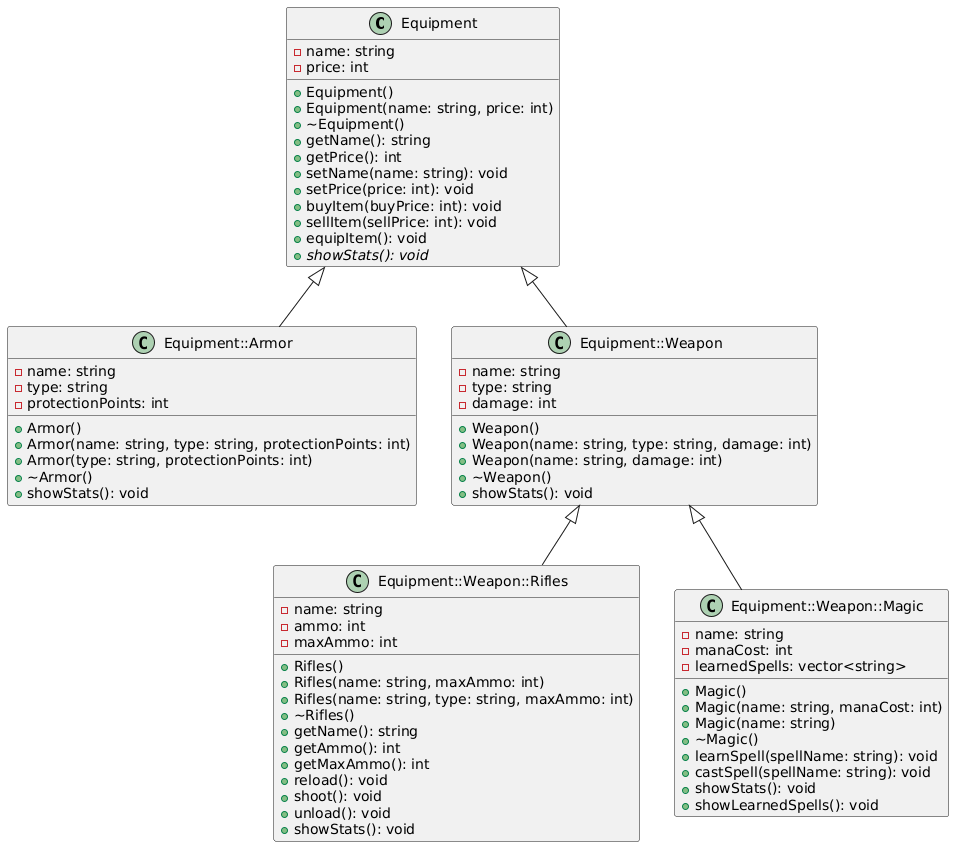
\includegraphics[width=0.58\textwidth]{1.png}
    \caption*{Рисунок \arabic{imgcnt} -- Диаграмма классов}
    \stepcounter{imgcnt}
\end{figure}

\newpage
\section*{\normalsize Вывод}
В ходе выполнения лабораторной работы были получены навыки реализации абстрактных классов, наследования, полиморфизма и инкапсуляции в C++. Создана иерархия классов, описывающая игровое снаряжение. Базовый класс \texttt{Equipment} является абстрактным благодаря чисто виртуальной функции \texttt{showStats()}. Классы-наследники предоставляют по три конструктора, переопределяют виртуальные методы и добавляют собственную функциональность. Продемонстрирована работа с полиморфным массивом, а также использование \texttt{static\_cast}, \texttt{dynamic\_cast} и C-приведения типов.

\end{document}